\documentclass[a4paper,12pt]{article}

\usepackage[english, russian]{babel}
\usepackage[utf8]{inputenc}
\usepackage{graphicx}
\usepackage{subfig}
\usepackage{amsmath}
\usepackage{listings}
\usepackage[top=2cm, bottom=1.5cm, left=2cm, right=1.5cm]{geometry}
\usepackage{mathtools}
\usepackage[numbered,framed]{matlab-prettifier}
\usepackage{filecontents}
\usepackage[T1]{fontenc}
\usepackage{listings,chngcntr}
\usepackage{float}

\begin{document}
%\counterwithin{lstlisting}{}
\thispagestyle{empty} %чтобы не было номера на первой странице

\begin{centering}
	\textbf{
{\large МИНОБРНАУКИ РОССИИ\\
САНКТ-ПЕТЕРБУРГСКИЙ ГОСУДАРСТВЕННЫЙ\\
ЭЛЕКТРОТЕХНИЧЕСКИЙ УНИВЕРСИТЕТ\\
«ЛЭТИ» ИМ. В.И. УЛЬЯНОВА (ЛЕНИНА)\\
Кафедра САПР}\\
}
\end{centering}


\vspace{7cm}

\begin{centering}
\textbf{{\large 
ЗАДАНИЕ\\
по лабораторной работе №2\\
по дисциплине «Методы оптимизации»\\
Тема: \guillemotleftМетоды одномерной оптимизации на основе поиска
стационарной точки\guillemotright\\
}}
\end{centering}

\vspace{4cm}

\begin{tabular}{l r}
    \textbf{{\large Студенты:}}&\hspace{6cm} \textbf{{\large Литвинов К.Л.}}\\
   \textbf{}&\hspace{6cm} \textbf{{\large Гарцев Е.А.}}\\
   \textbf{{}}&\hspace{6cm} \textbf{\large{Бурков М.П.}}\\
    \textbf{{\large Преподаватель:}}&\hspace{6cm} \textbf{{\large Каримов А.И.}}\\
\end{tabular}

\vspace{6cm}


\begin{centering}
	{\large
Санкт-Петербург \\
2019 \\
}
\end{centering}

\newpage
 
\subsection*{Цель работы}

Изучение среды MATLAB, создание программы для реализации двух 
методов одномерного поиска на основе поиска стационарной точки: 

\begin{itemize}
	\item Метод секущих;
    \item Метод Трёхточечного деления;
\end{itemize}


\subsection*{Основные теоретические положения}

Критические и стационарные точки функции определяются следующим образом.

\textbf{Критические точки} функции $f(x)$ -- точки, в которых производная $f'(x)$ не существует или обращается в нуль.

\textbf{Стационарные точки} функции $f(x)$ -- точки, в которых производная $f'(x)$ обращается в нуль.

При этом стационарные точки подрязделяются на:

\begin{itemize}
	\item экстремумы -- точки минимума или максимума;
	\item седловые точки -- точки, в которых производная нулевая, но минимум или максимум не достигается.
\end{itemize}


\textbf{Лемма Ферма} утверждает: производная $f'(x)$ дифференцируемой функции в точке экстремума равна нулю.
В соответствии с этой леммой, возможно использования метода нахождения нуля производной в качестве метода оптимизации. Для этого осуществляются следующие шаги:

1) Поиск ${x_i^*}: f''(x^*) = 0$

2) Осуществляется проверка: $x_i^*$ -- экстремум, если  

\begin{equation}
f'''(x^*) \neq 0
\label{lf1}
\end{equation}

 или 
 
 \begin{equation}
  f''(x^* - \epsilon)f''(x^* + \epsilon) < 0, 
  \label{lf2}
 \end{equation}
где $\epsilon > 0$ -- малое число (взаимозаменяемые условия).


\subsubsection*{Метод секущих}

Метод секущих предлагает заменить вторую производную 
$f''(x_k)$ в ньютоновской формуле её линейной аппроксимацией $(f'(x_k) - f'(x_{k - 1}))/(x_{k} - x_{k - 1})$. Тем самым,

\begin{equation*}
x_{k + 1} = x_k - \frac{f'(x_k)(x_k - x_{k - 1})}{f'(x_k) - f '(x_{k – 1})}.
\end{equation*}

Легко видеть, что $x_{k + 1}$ -- точка пересечения с осью абсцисс секущей прямой, проходящей через точки $x_{k}$ и $x_{k - 1}$.

\textbf{Псевдокод}

\textbf{Цикл} 

$x_{k + 1} = b_{k} - f'(b_k)(b_k - a_k)/(f'(b_k) - f'(a_k))$; 

\textbf{Если}

\quad $|f'(x_{k + 1})| \leq \epsilon$, \textcolor{gray}{//КОП}

\textbf{то}

\quad остановиться

\textbf{иначе} \textcolor{gray}{// Уменьшить интервал поиска минимума}


\quad \textbf{Если}

\quad\quad $ f'(x_{k + 1}) > 0$, 

\quad \textbf{то}

\quad\quad$a_{k + 1} = a_k$, $b_{k + 1} = x_{k + 1},$ 

\quad\textbf{иначе}


\quad\quad$a_{k + 1} = x_{k + 1}$, $b_{k + 1} = b_k$;


$k = k + 1$;


\textbf{Пока не выполнен КОП}

\subsection*{Код программы}
\begin{lstlisting}[style=Matlab-editor, caption=Метод Трёхточечного деления]
function [xm, k] = ThreeDots(dfunction,funct , a, b, tol) 
    format long g
    t = a:0.1:b; k = 1;
    epsilon = tol; delta = tol;
    %Visualization
    deltaX = (b-a)/100;
    figure(3); hold on
    [miny, maxy] = drawplot(dfunction,funct,a,b,a,b,k); %drawing plot of the function and derivative
    deltaY = abs(maxy - miny)/100;
    k = 0;
    print('-dpdf',[num2str(k), 'ThreeDotsIter'])
    %Main algorithm
    xk = (a + b) / 2;
    %Three dots method
    xm = (a+b)./2;
    Lk = abs(b-a);
    x1 = (a+Lk/4);
    x2 = (b-Lk/4);
    while Lk>epsilon & k < 5
        if funct(x1)<funct(xm)
            b = xm;
            xm = x1;
        elseif (funct(x1)>=funct(xm)) & (funct(xm)<=funct(x2))
            a = x1;
            b = x2;
        else
            a = xm;
            xm = x2;
        end
        k = k + 1;
        xm = (a+b)./2;
        Lk = abs(b-a);
        x1 = (a+Lk/4);
        x2 = (b-Lk/4);
        drawplot(dfunction,funct,a,b,x1, x2 ,k);
        print('-dpdf',[num2str(k), 'ThreeDotsIter'])
    end 
    x1, x2

    hold off
end

function [miny maxy] = drawplot(df, f, a, b, x1, x2, iternumber)
    
    figure(3); 
    h = (b-a)/100;
    %Drawing plot of dfunction
    dx = a:h:b;
    dy = feval(f,dx);
    miny = min(dy);
    maxy = max(dy);
    deltaX = (b-a) / 100;
    deltaY = abs(maxy - miny)/100;
    colp = hsv2rgb([rand(), 1, 0.5+0.5*rand()]);
    col = hsv2rgb([rand(), 1, 0.5+0.5*rand()]);
    %Drawing plot of the function
    x = a:h:b;
    y = feval(f,x);
    plot(x, y, 'LineWidth', 1, 'Color', colp);
    %xlim([2.8 3.4])
    line([a b],[-50 -50],'Color','k','LineWidth',1); %axis x
    ylim([-55 -30])
    xlabel('\itx')
    ylabel('\it{}f\rm (\it{}x\rm)')
    hold on
    line([x1 x1],[-50 feval(f, x1)],'Marker','s','Color',col,'LineWidth',1,'MarkerSize',4); 
    scatter(x1,feval(f, x1),'Marker','o','MarkerFaceColor',colp,'MarkerEdgeColor',colp);
    line([x2 x2],[-50 feval(f, x2)],'Marker','s','Color',col,'LineWidth',1,'MarkerSize',4); 
    scatter(x2,feval(f, x2),'Marker','o','MarkerFaceColor',colp,'MarkerEdgeColor',colp);
    textColor = 'black';
    textBackground = 'white';
    text(x1 - deltaX/2, feval(f, x1) + 4*deltaY + 1, num2str(iternumber),'Color', textColor,'BackgroundColor', textBackground);
    text(x2 - deltaX/2, feval(f, x2) + 4*deltaY + 1, num2str(iternumber));
    input("");
end
\end{lstlisting}

\subsection*{Графики, демонстрирующие работу метода трёхточеченого деления}
    \begin{figure}[H]
        \centering
        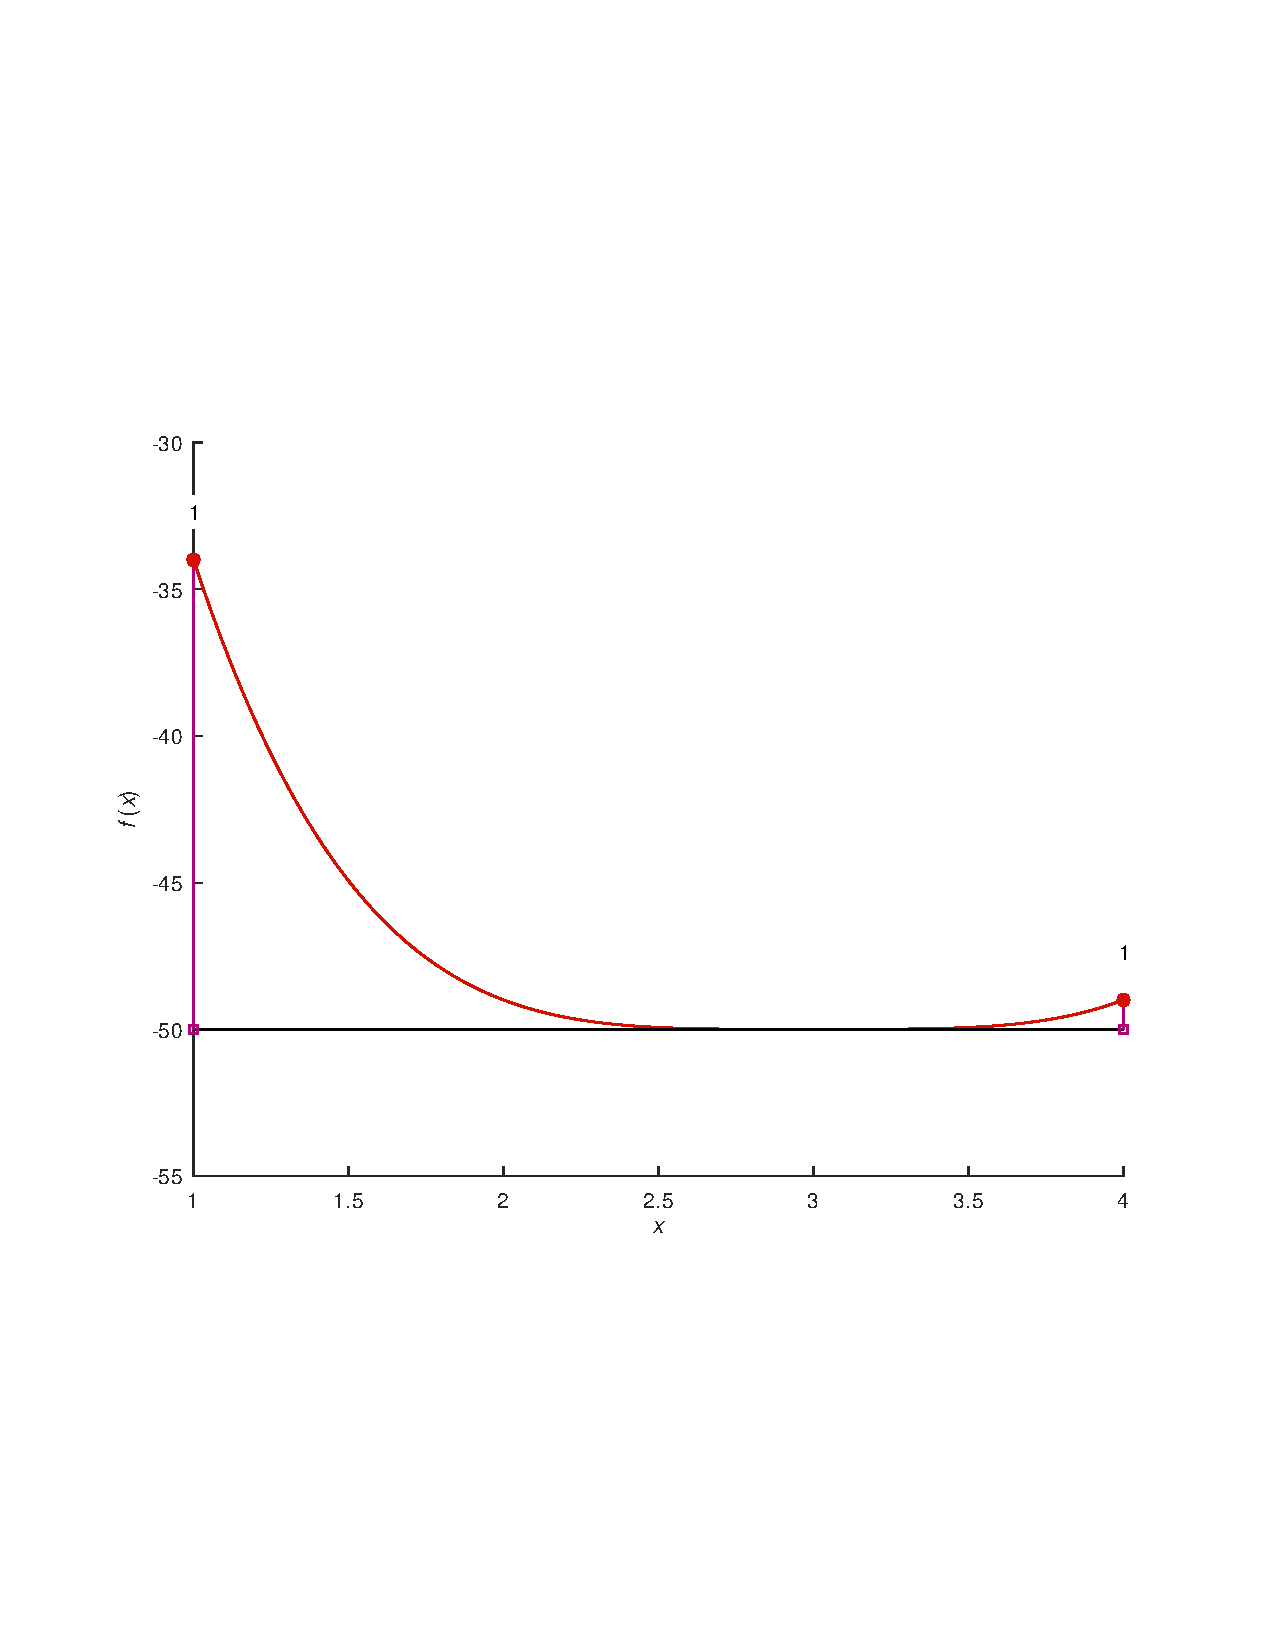
\includegraphics[scale=0.4]{0Bolcanoitter.pdf}
        \caption{инициализация}
    \end{figure}
    \begin{figure}[H]
        \centering
        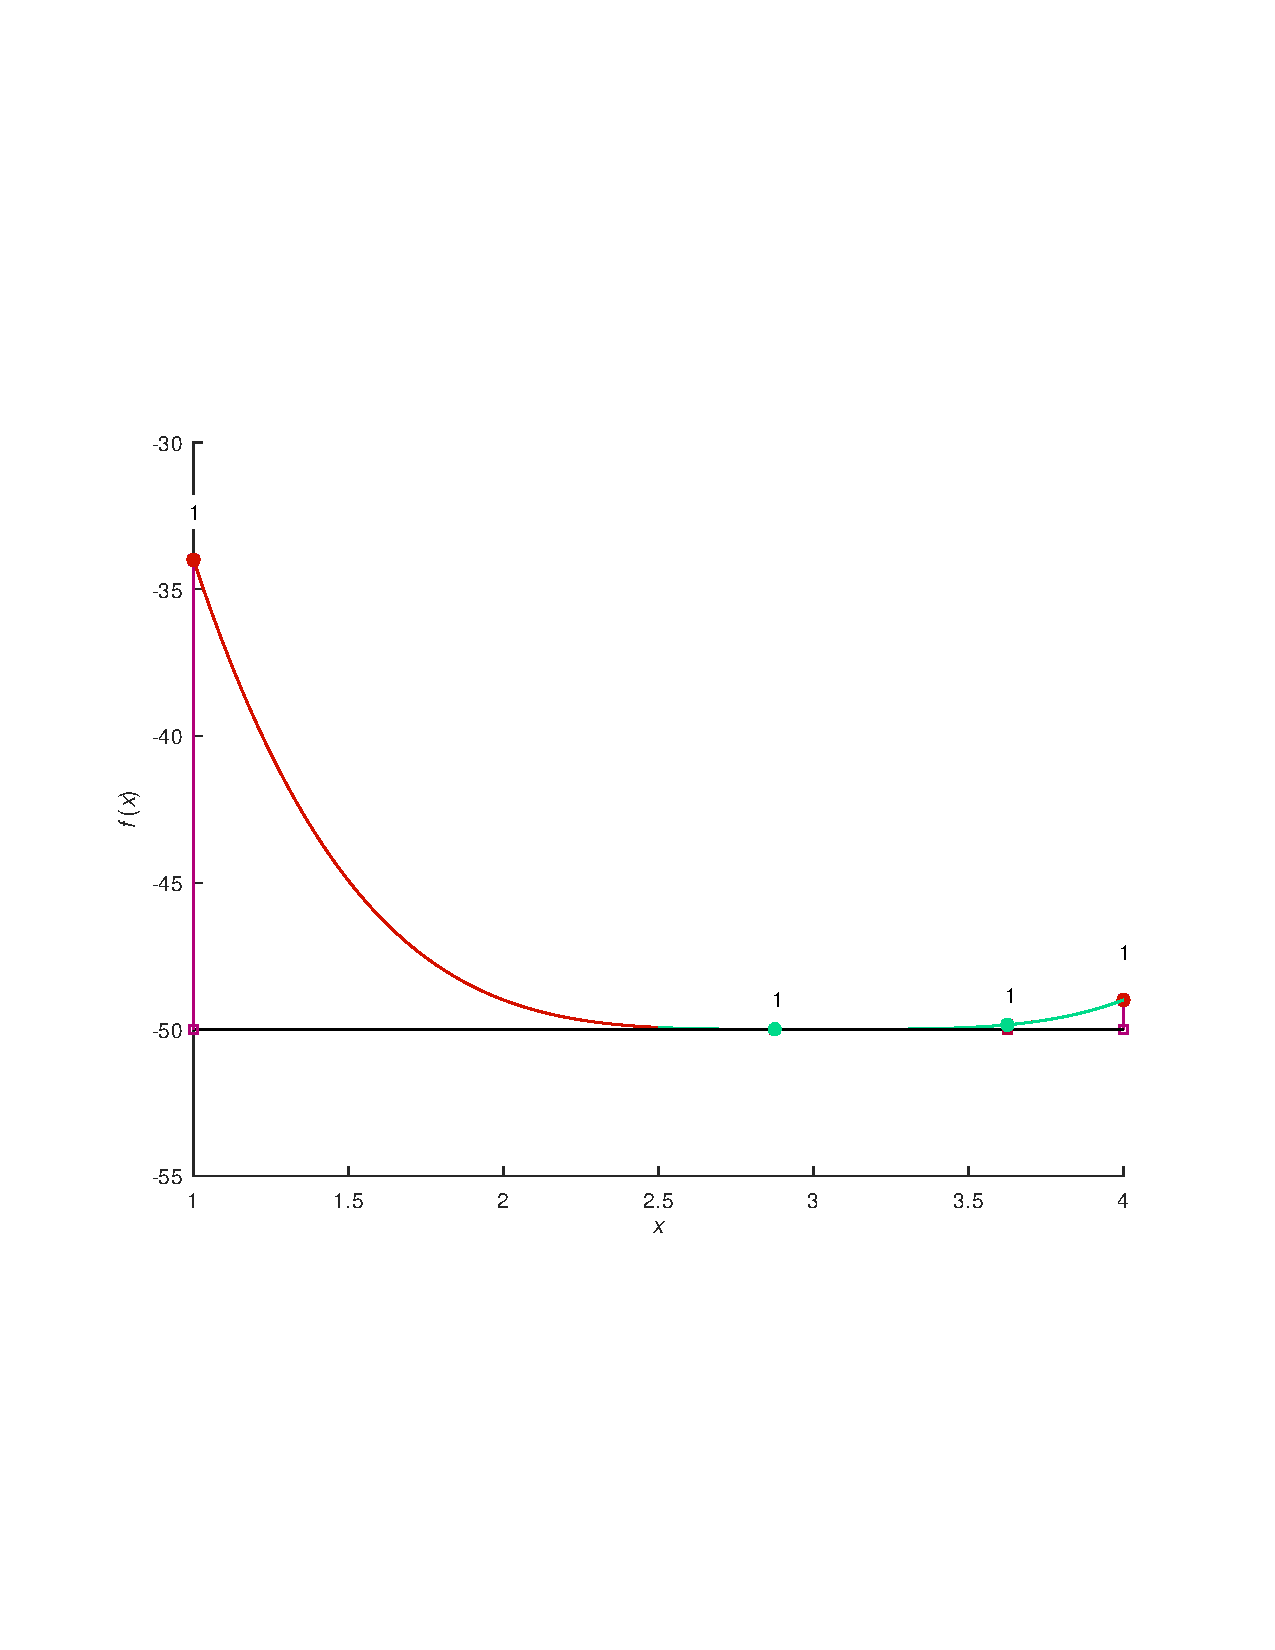
\includegraphics[scale=0.4]{1Bolcanoitter.pdf}
        \caption{Первая итерация}
    \end{figure}
    \begin{figure}[H]
        \centering
        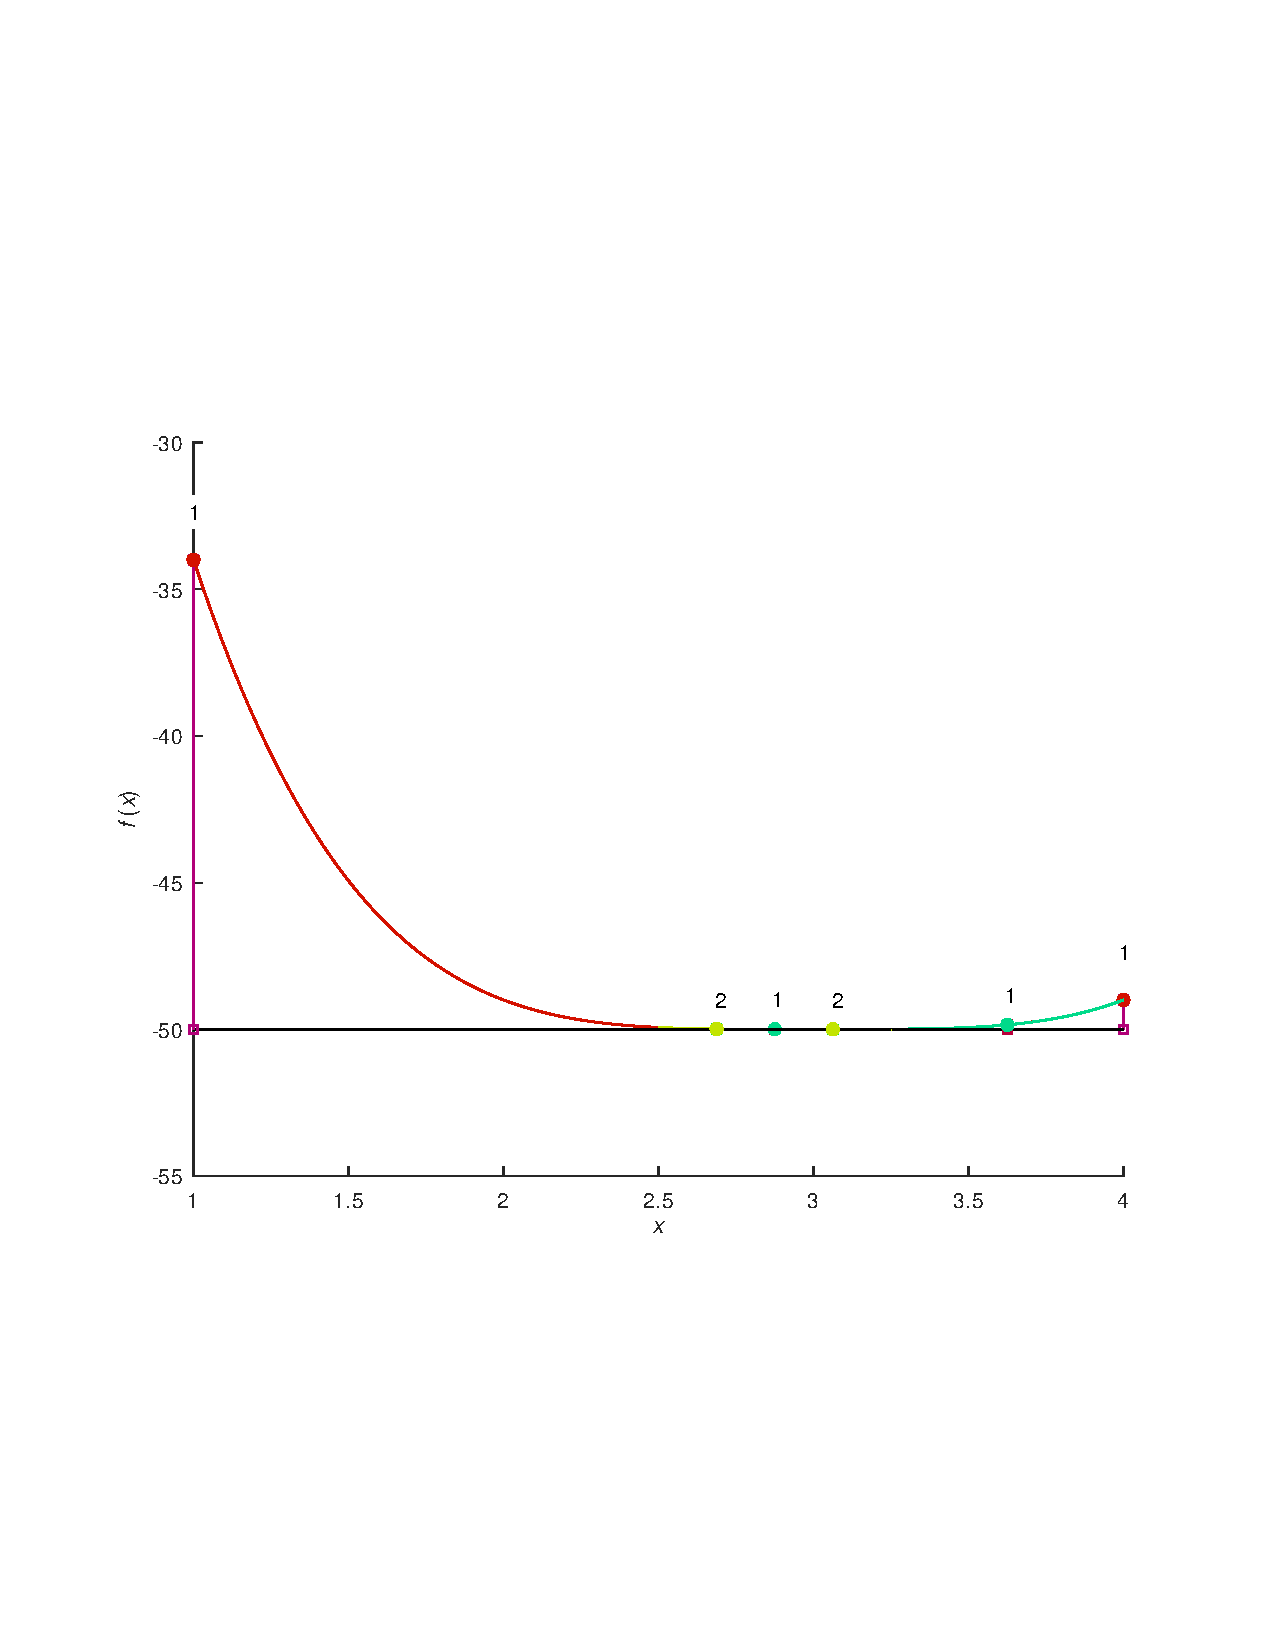
\includegraphics[scale=0.4]{2Bolcanoitter.pdf}
        \caption{Вторая итерация}
    \end{figure}
    \begin{figure}[H]
        \centering
        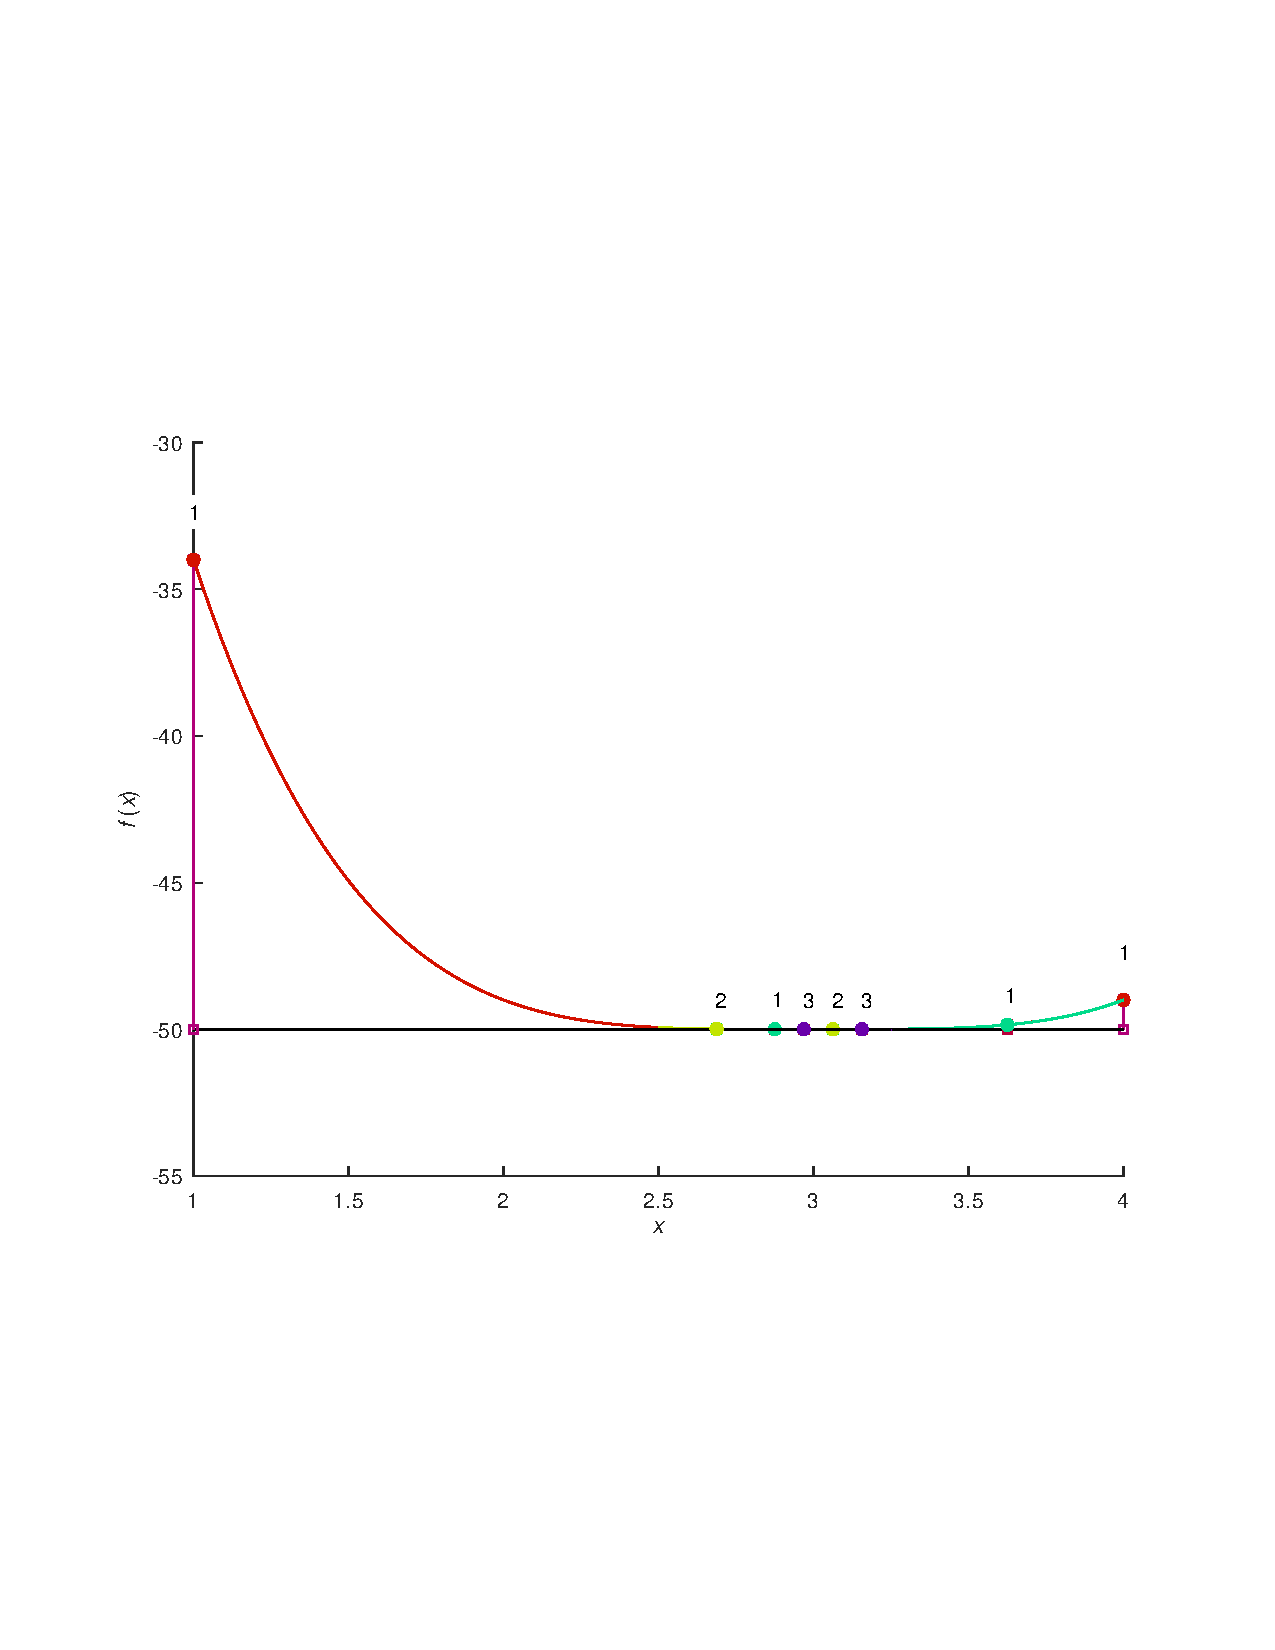
\includegraphics[scale=0.4]{3Bolcanoitter.pdf}
        \caption{Третья итерация}
    \end{figure}
    \begin{figure}[H]
        \centering
        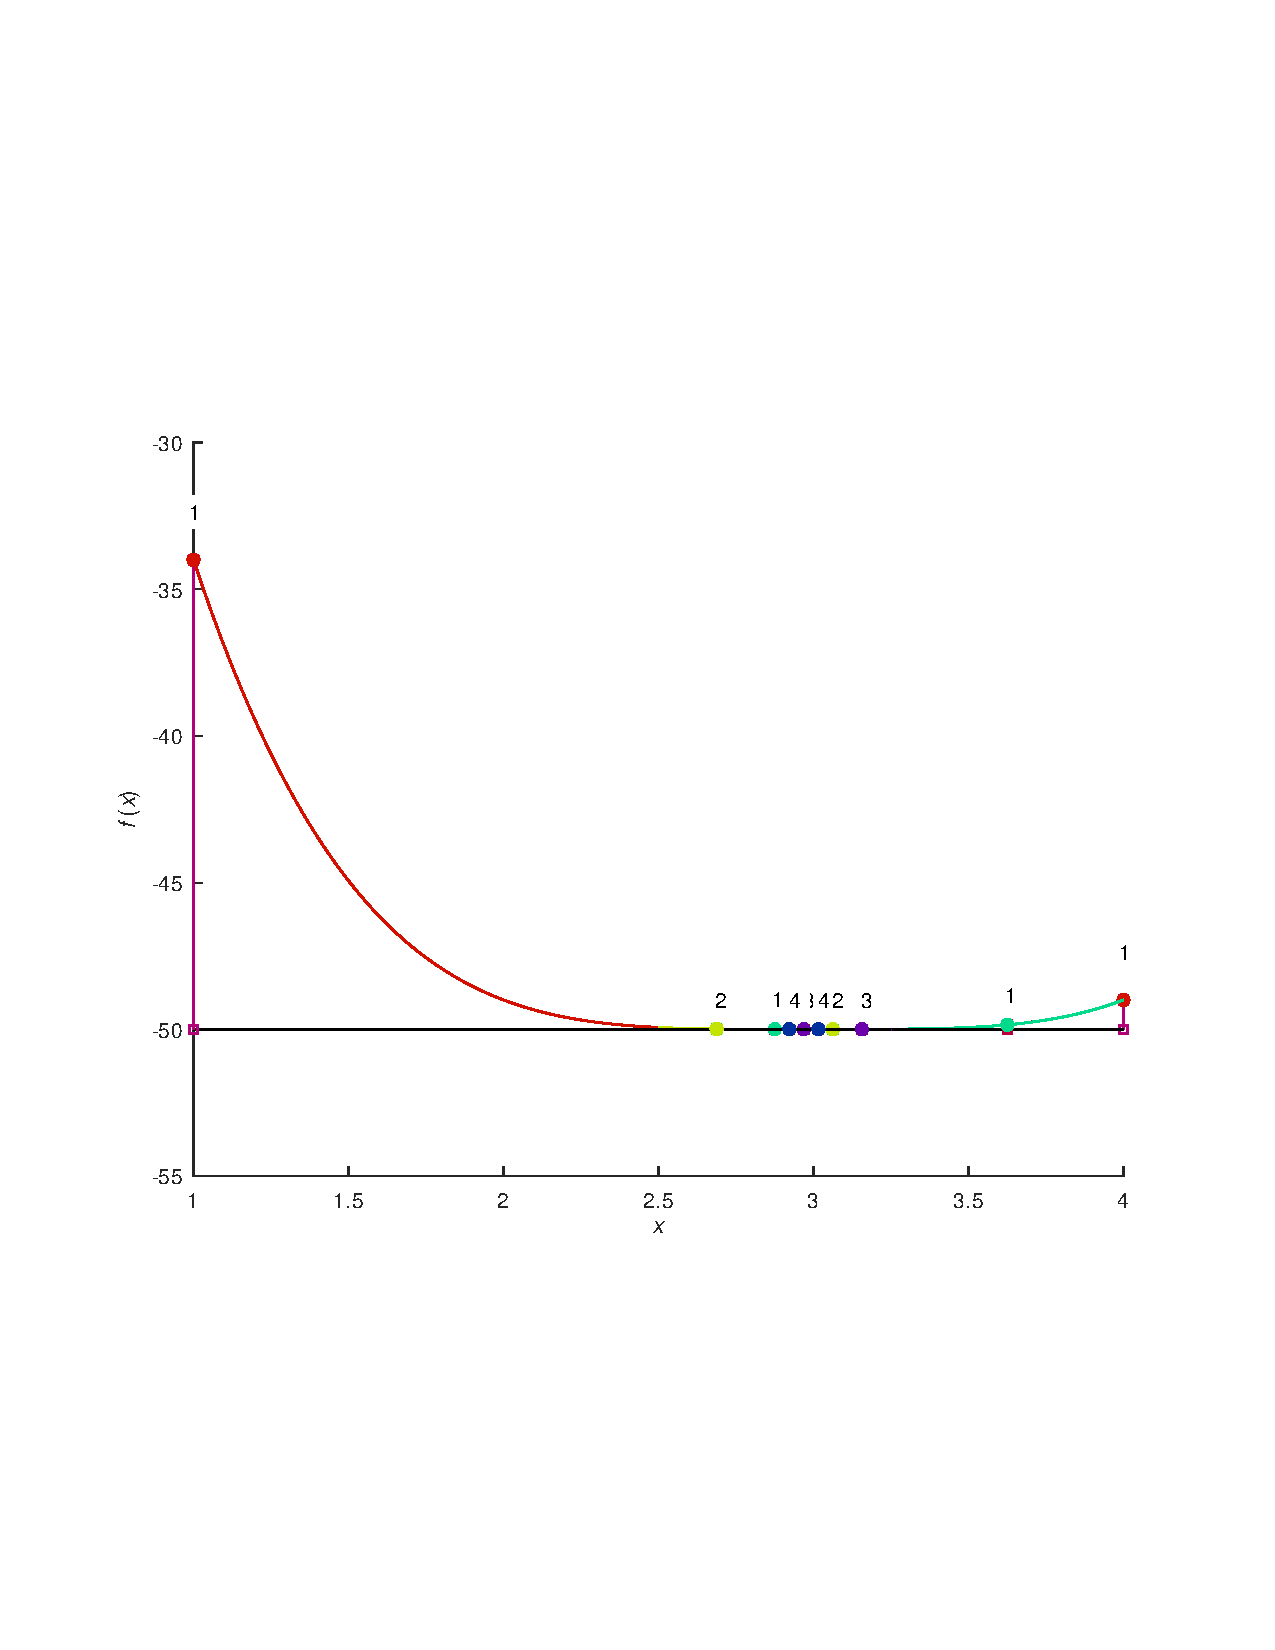
\includegraphics[scale=0.4]{4Bolcanoitter.pdf}
        \caption{Четвёртая итерация}
    \end{figure} 
    \begin{figure}[H]
        \centering
        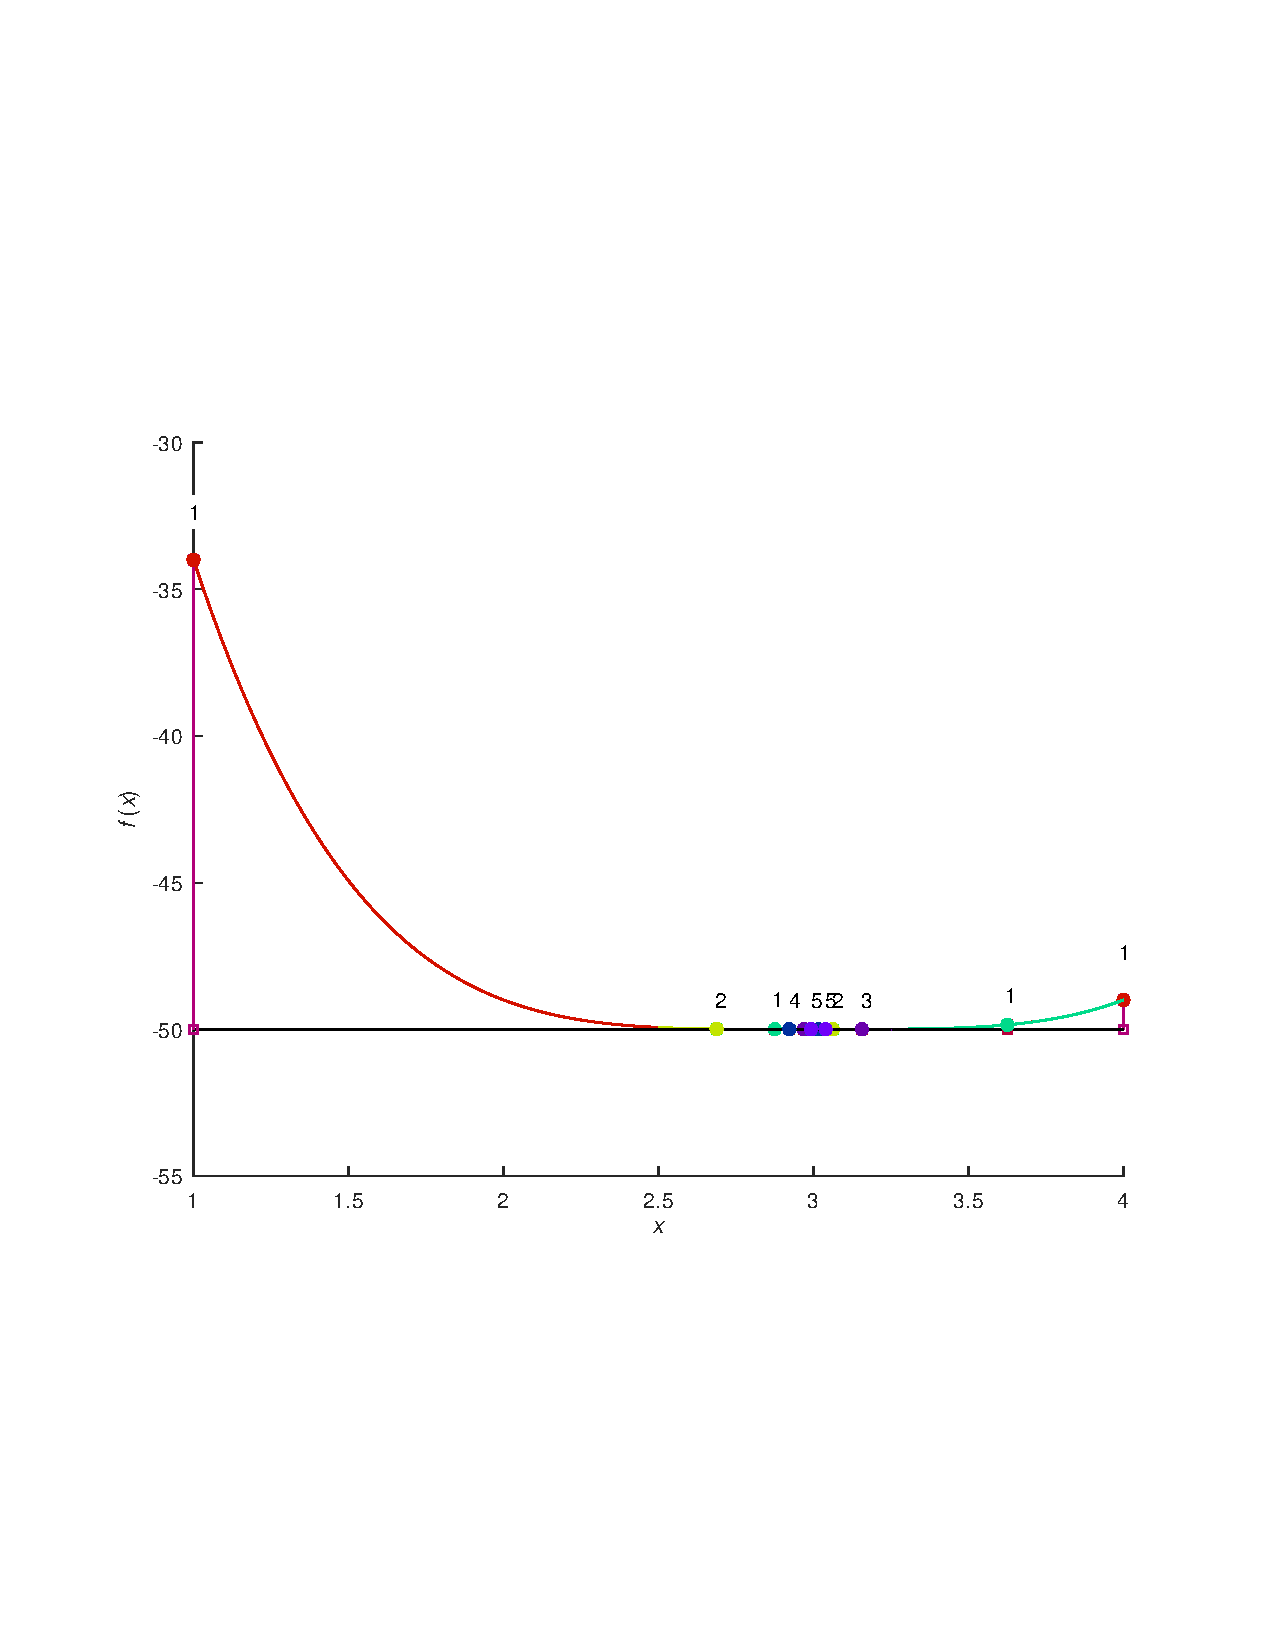
\includegraphics[scale=0.4]{5Bolcanoitter.pdf}
        \caption{Пятая итерация}
    \end{figure}     
\newpage
\\
\subsection*{Код метода секущих}
\begin{lstlisting}[style=Matlab-editor, caption=Метод секущих]
function [xk, k] = secant(dfunction, funct, a, b, tol)
    epsilon = tol;
    %Visualization
    deltaX = a:(b-a) / 100:b;
    figure(3); 
    k = 0;
    [miny, maxy] = drawplot(dfunction,funct,a,b,a, k); %drawing plot of the function and derivative
    deltaY = abs(maxy - miny)/100;
    print('-dpdf',[num2str(k), 'secantitter'])
    %Secant method
    while 1
        xk = b - dfunction(b)*(b - a) / (dfunction(b) - dfunction(a));
        if abs(dfunction(xk)) <= epsilon | k > 6
            break
        else
            dfunction(xk), xk
            if dfunction(xk) > 0
                b = xk;
            else
                a = xk;
            end
        end
        subplot(2,1,1);
        k = k + 1;
        drawplot(dfunction, funct, a, b, xk, k);
        print('-dpdf',[num2str(k), 'secantitter'])
    end
hold off
end

function [miny maxy] = drawplot(df, f, a, b, x1, iternumber)
    
    figure(3); 
    h = (b-a)/100;
    %Drawing plot od dfunction
    dx = a:h:b;
    dy = feval(df,dx);
    miny = min(dy);
    maxy = max(dy);
    deltaX = (b-a) / 100;
    deltaY = abs(maxy - miny)/100;
    subplot(2,1,1);
    colp = hsv2rgb([rand(), 1, 0.5+0.5*rand()]);
    col = hsv2rgb([rand(), 1, 0.5+0.5*rand()]);
    plot(dx,dy,'LineWidth',1,'Color',colp);
    xlim([2.5 4])
    ylim([-10 20])
    xlabel('\itx')
    ylabel('\it{}df\rm (\it{}x\rm)')
    hold on
    scatter([a b],[feval(df,a), feval(df,b)],'Marker','o','MarkerFaceColor',colp,'MarkerEdgeColor',colp);
    line([a b],[0 0],'Color','k','LineWidth',1); %axis x
    y1 = feval(df, x1);
    ya = feval(df, a);
    yb = feval(df, b);
    %Deciding where to draw secant 
    if x1 == a
        line([a b],[ya yb],'Marker','s','Color',col,'LineWidth',1,'MarkerSize',4); %drawing secant
        line([a a],[0 feval(df, a)],'Marker','s','Color',col,'LineWidth',1,'MarkerSize',4);
        text(a - deltaX/2, feval(df, a) + 4*deltaY, num2str(iternumber));
    else
        line([a b],[ya yb],'Marker','s','Color',col,'LineWidth',1,'MarkerSize',4); %drawing secant
        line([b b],[0 feval(df, b)],'Marker','s','Color',col,'LineWidth',1,'MarkerSize',4);
        text(b - deltaX/2, feval(df, b) + 4*deltaY, num2str(iternumber));
    end
    %Drawing plot of the function
    x = a:h:b;
    y = feval(f,x);
    subplot(2,1,2);
    plot(x, y, 'LineWidth', 1, 'Color', colp);
    xlim([2.5 4])
    ylim([-60 -45])
    xlabel('\itx')
    ylabel('\it{}f\rm (\it{}x\rm)')
    hold on
    scatter(b, feval(f,b), 'Marker', 'o', 'MarkerFaceColor', colp, 'MarkerEdgeColor', colp);
    input("");
end
\end{lstlisting}

\subsection*{Графики, демонстрирующие работу метода секущих}
    \begin{figure}[H]
        \centering
        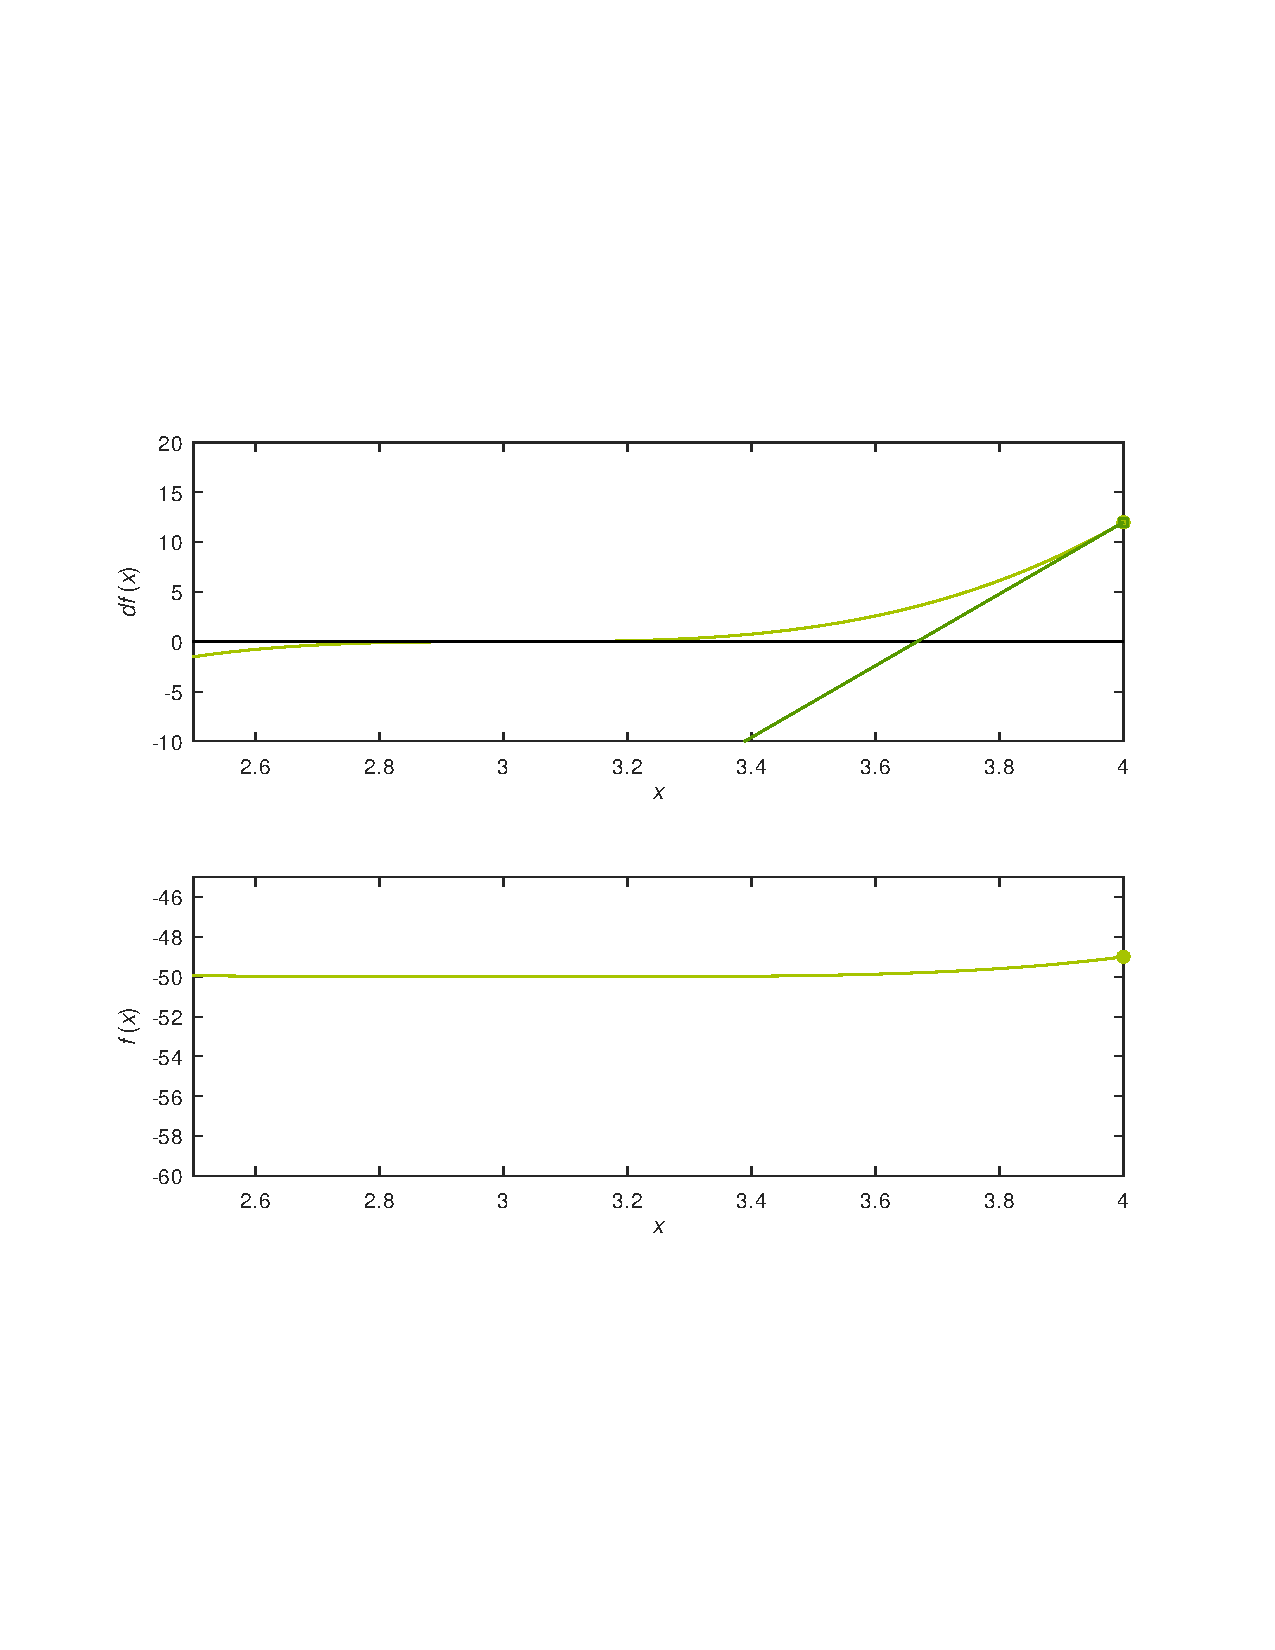
\includegraphics[scale=0.4]{0secantitter.pdf}
        \caption{инициализация}
    \end{figure}
    \begin{figure}[H]
        \centering
        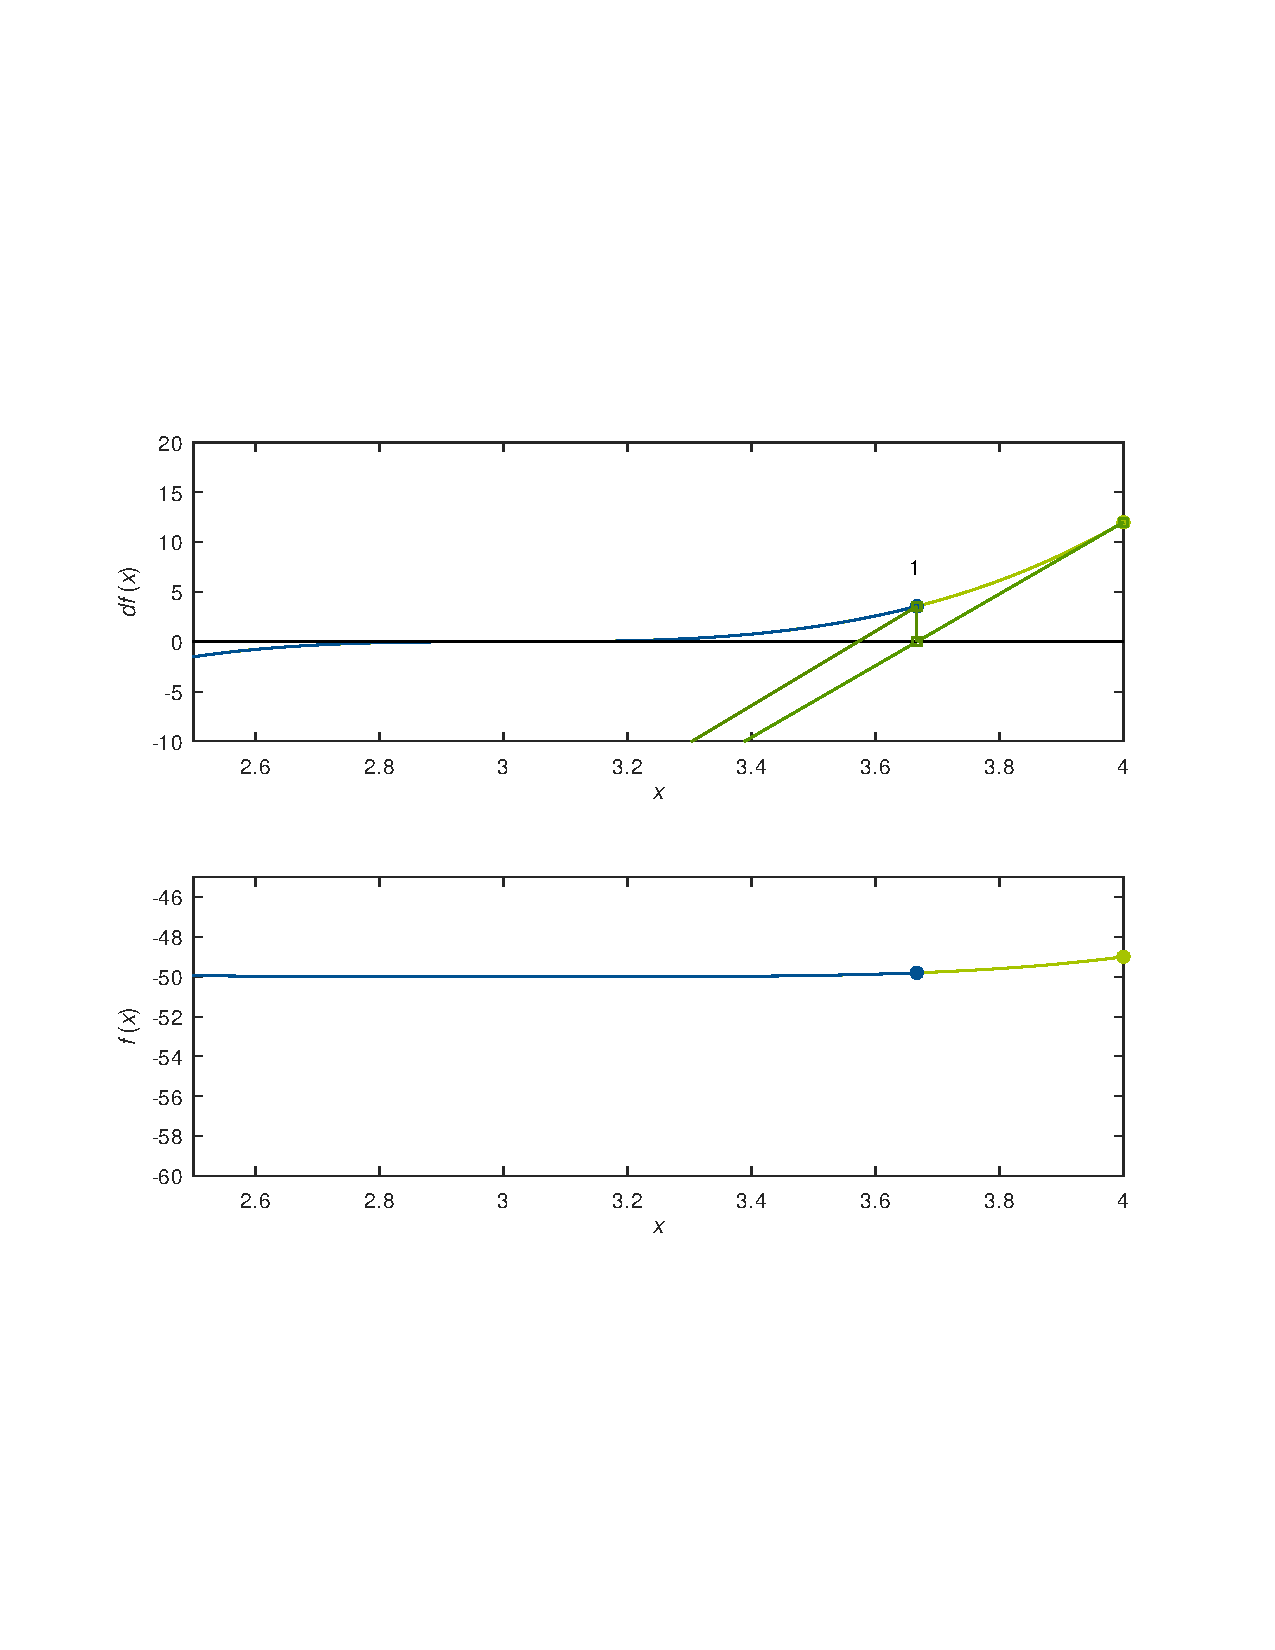
\includegraphics[scale=0.4]{1secantitter.pdf}
        \caption{Первая итерация}
    \end{figure}
    \begin{figure}[H]
        \centering
        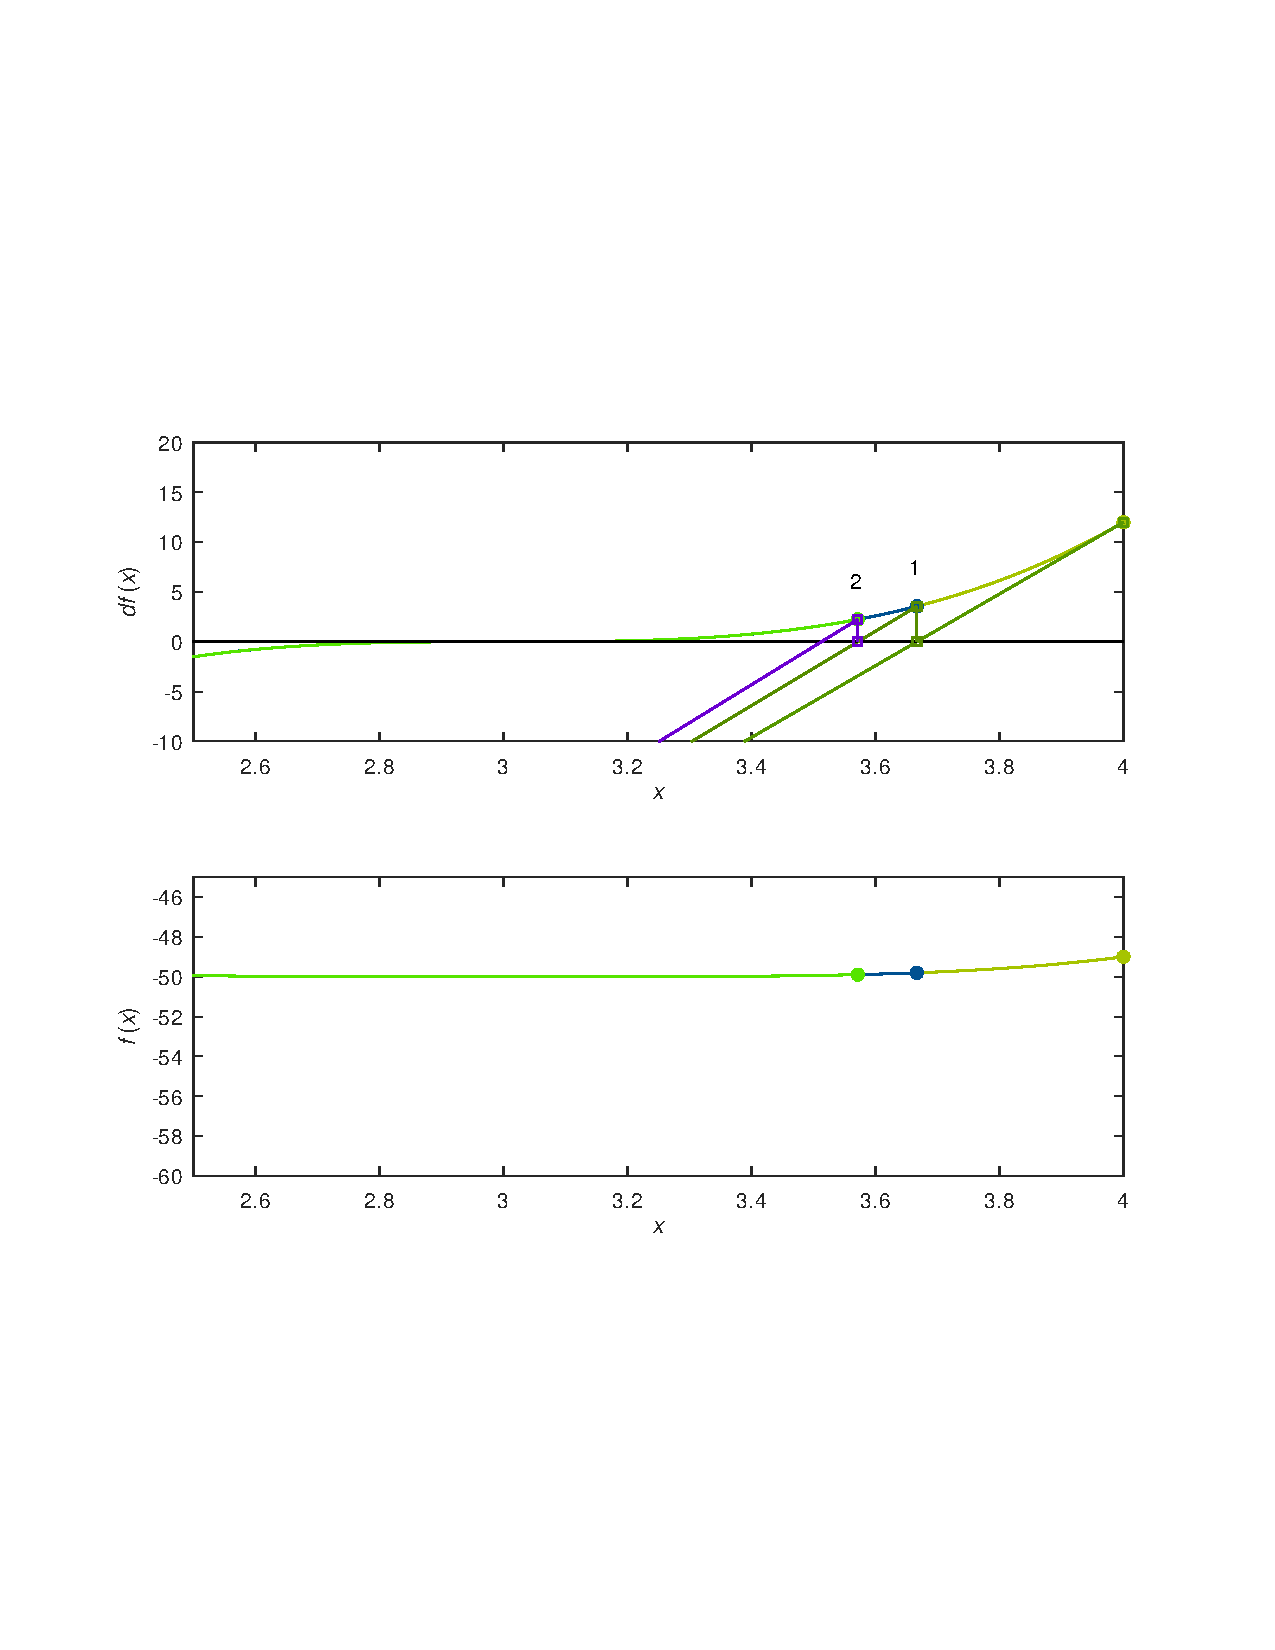
\includegraphics[scale=0.4]{2secantitter.pdf}
        \caption{Вторая итерация}
    \end{figure}
    \begin{figure}[H]
        \centering
        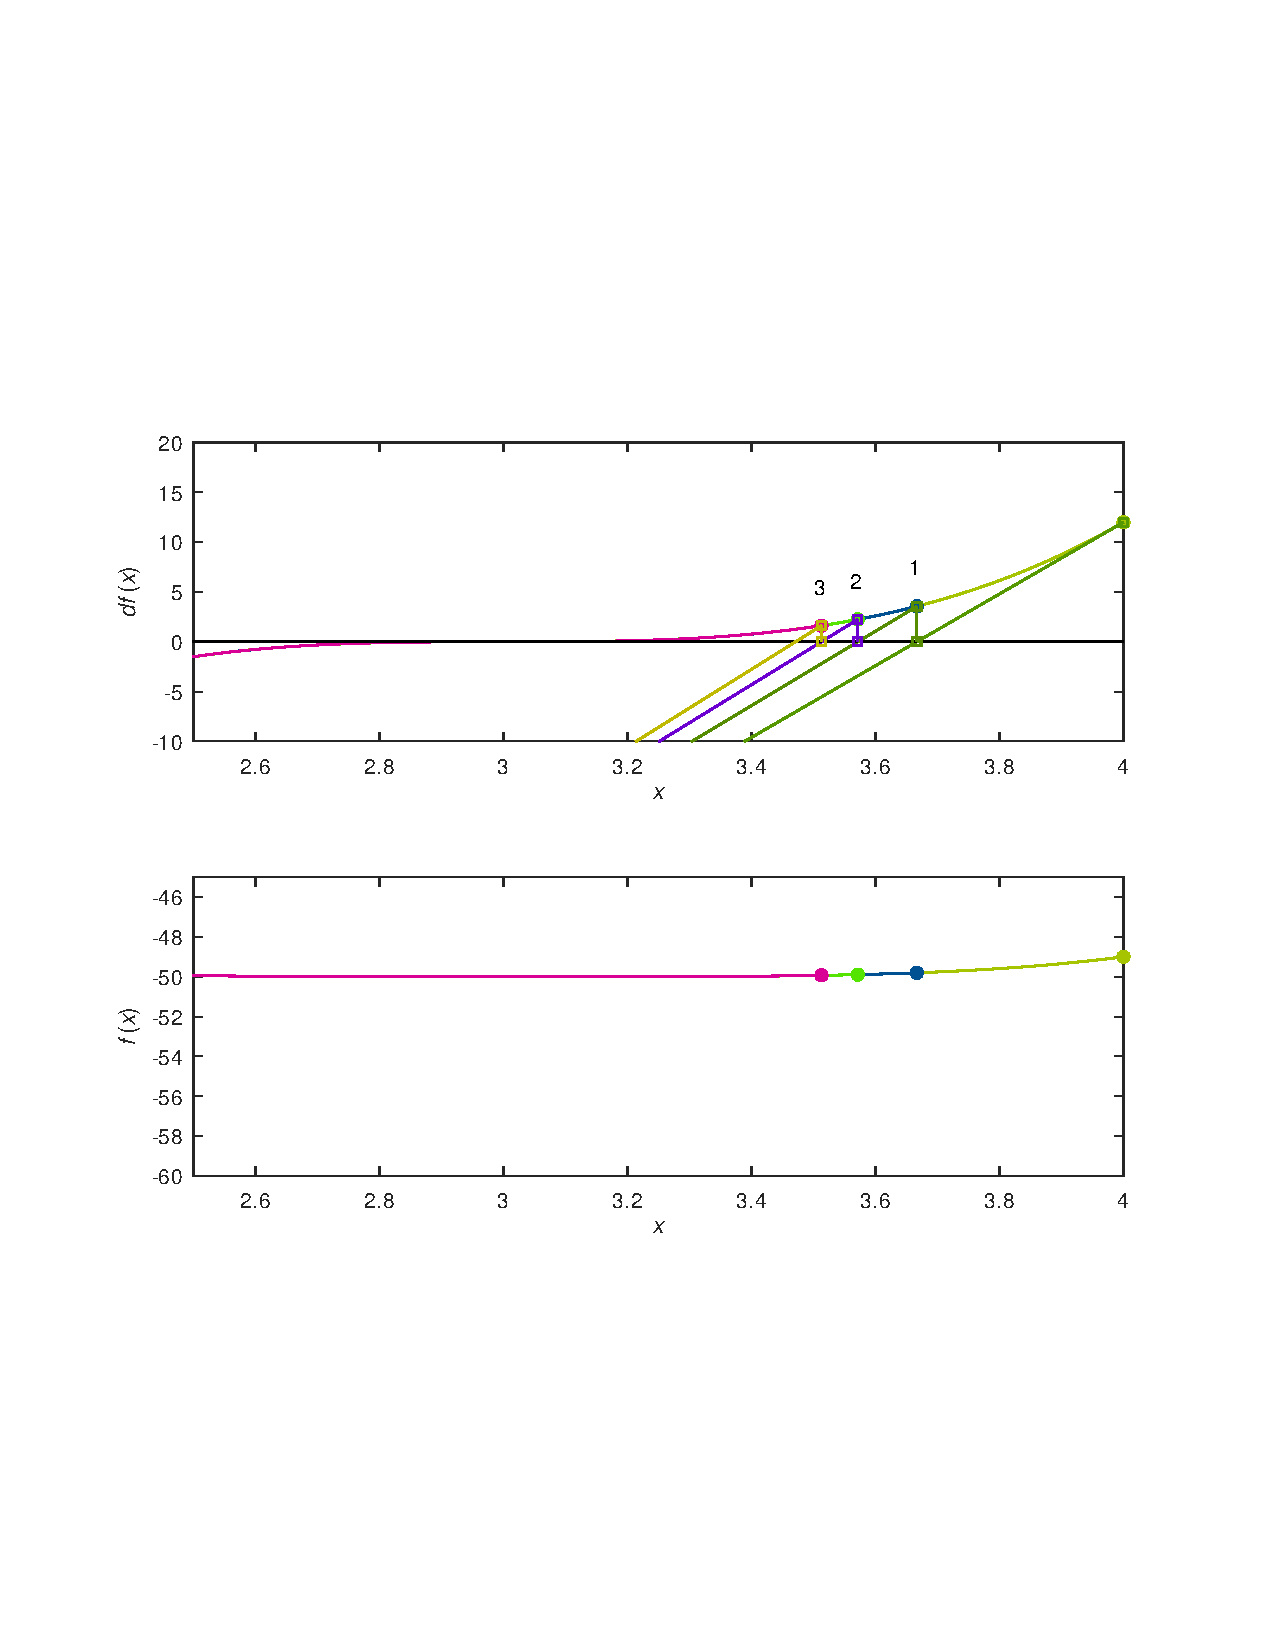
\includegraphics[scale=0.4]{3secantitter.pdf}
        \caption{Третья итерация}
    \end{figure}
    \begin{figure}[H]
        \centering
        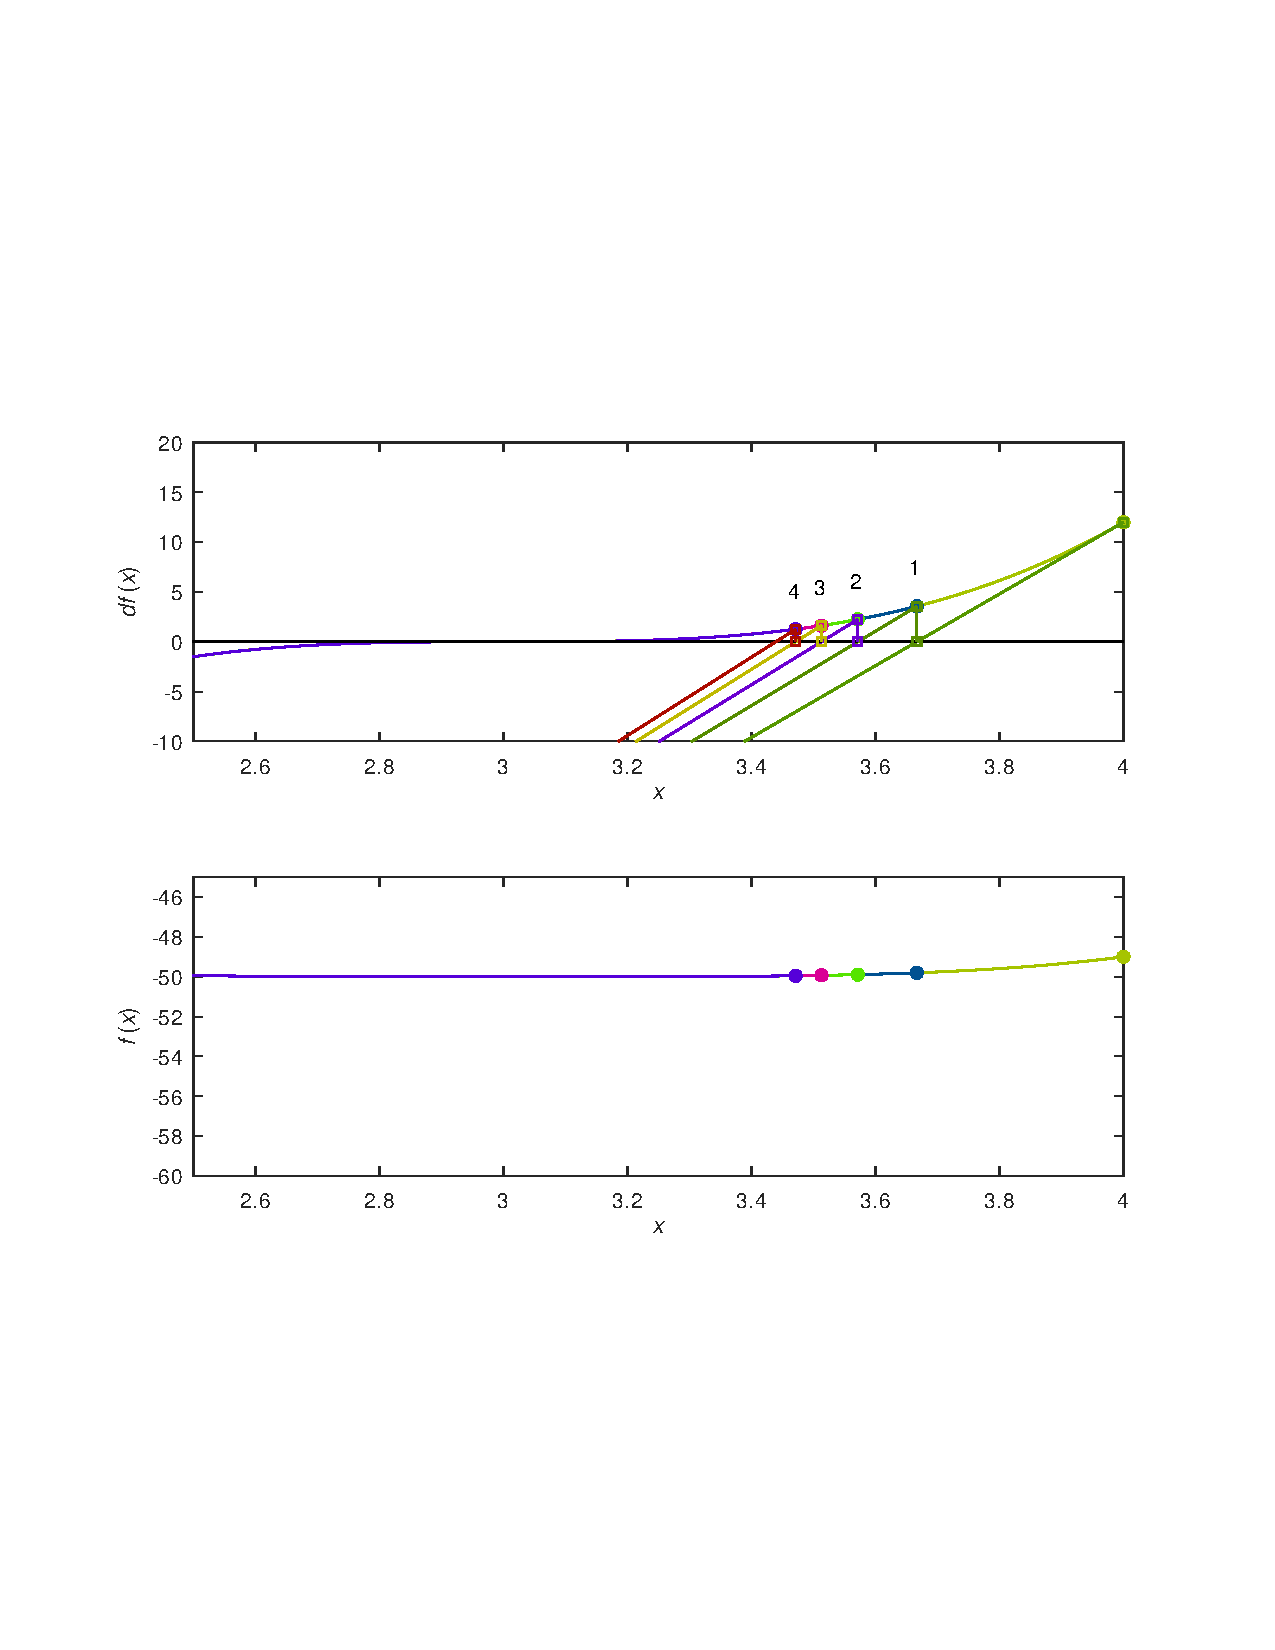
\includegraphics[scale=0.4]{4secantitter.pdf}
        \caption{Четвёртая итерация}
    \end{figure}
    \begin{figure}[H]
        \centering
        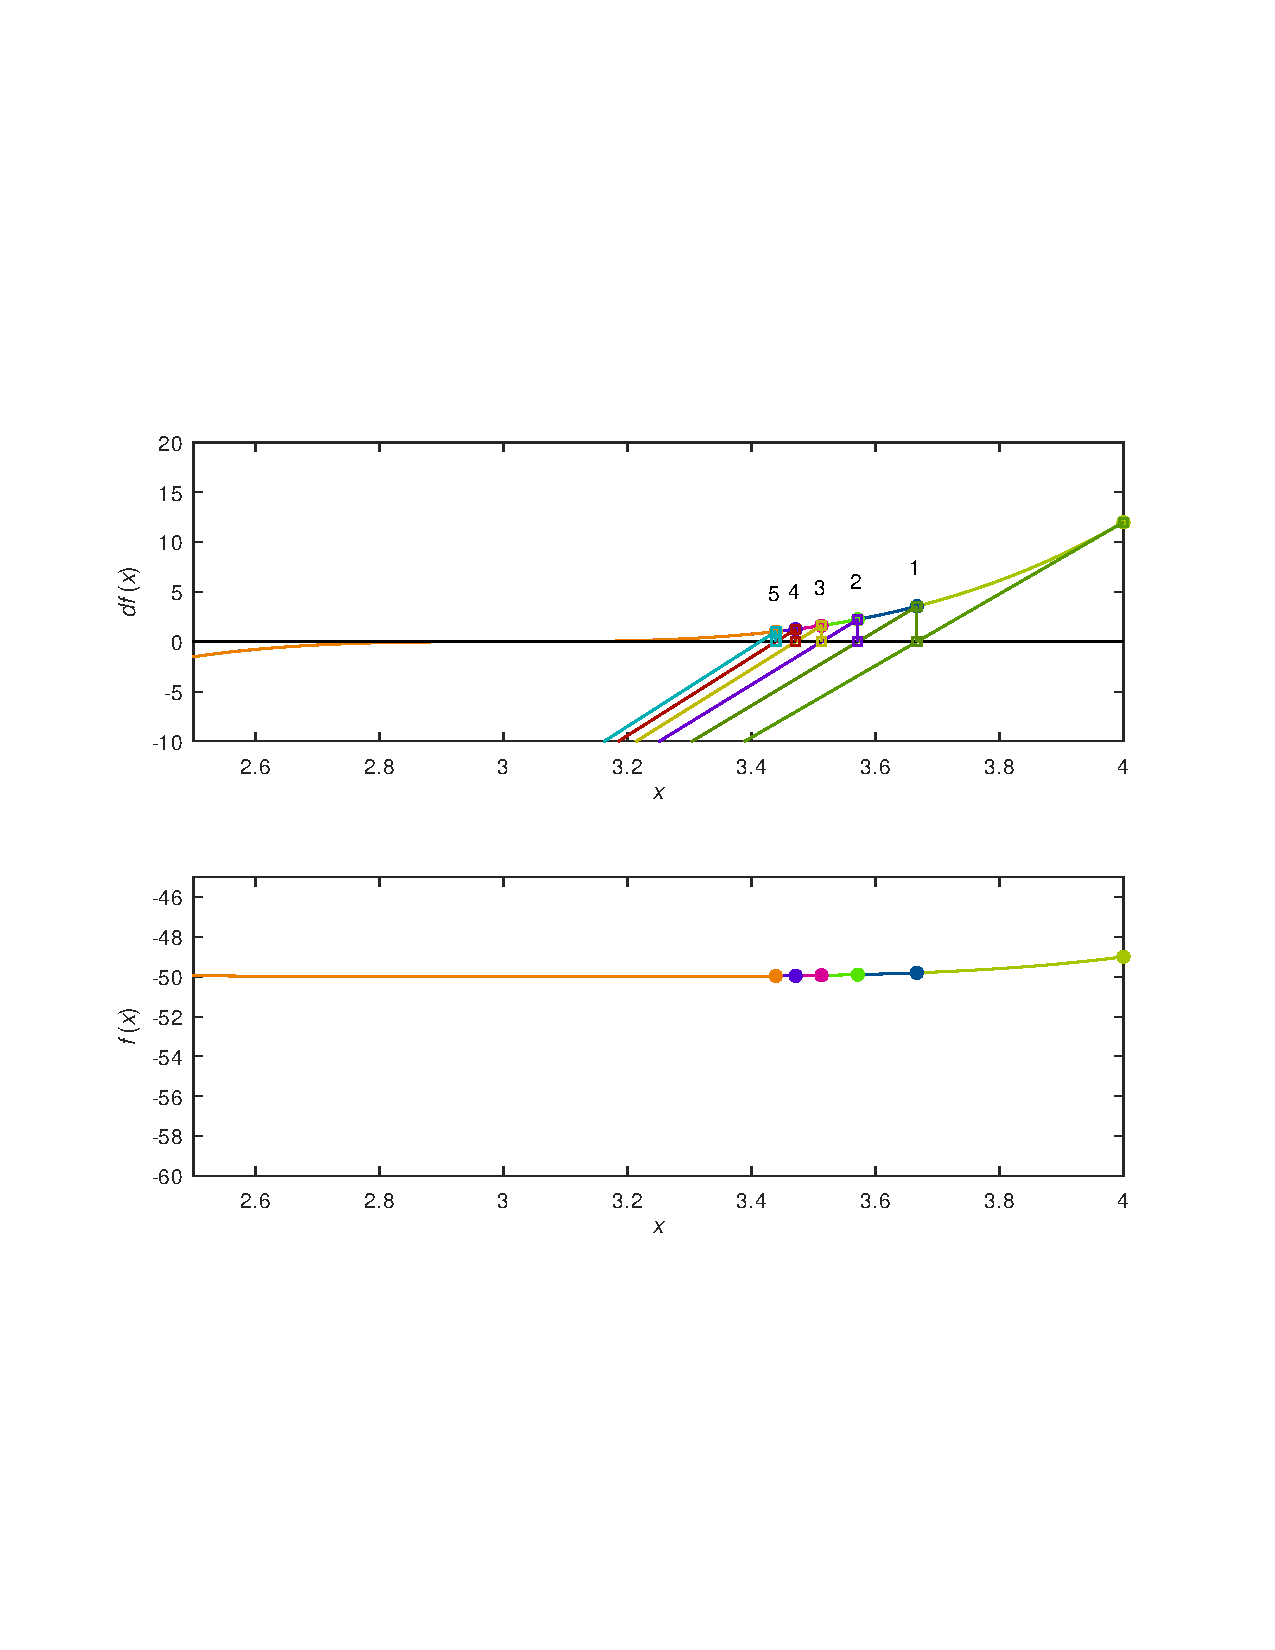
\includegraphics[scale=0.4]{5secantitter.pdf}
        \caption{Пятая итерация}
    \end{figure}
    \begin{figure}[H]
        \centering
        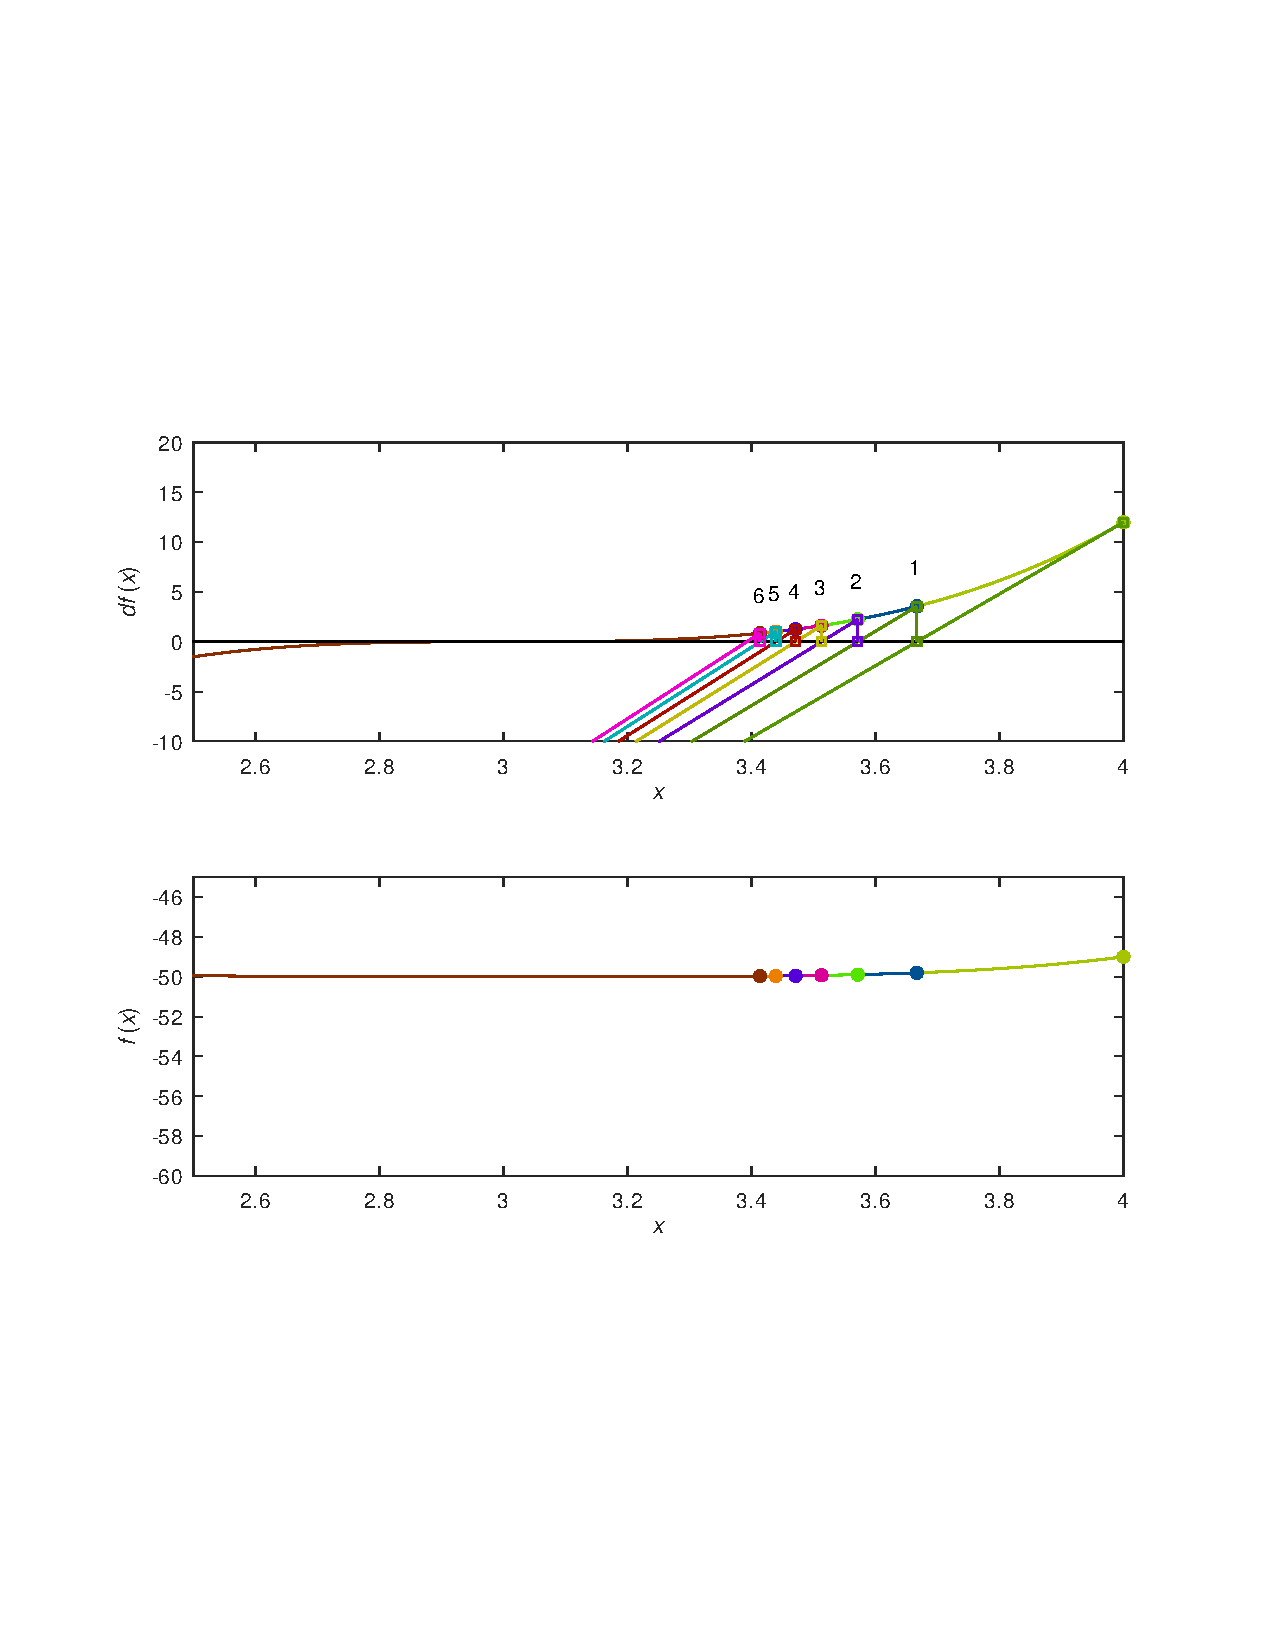
\includegraphics[scale=0.4]{6secantitter.pdf}
        \caption{Шестая итерация}
    \end{figure}
    \begin{figure}[H]
        \centering
        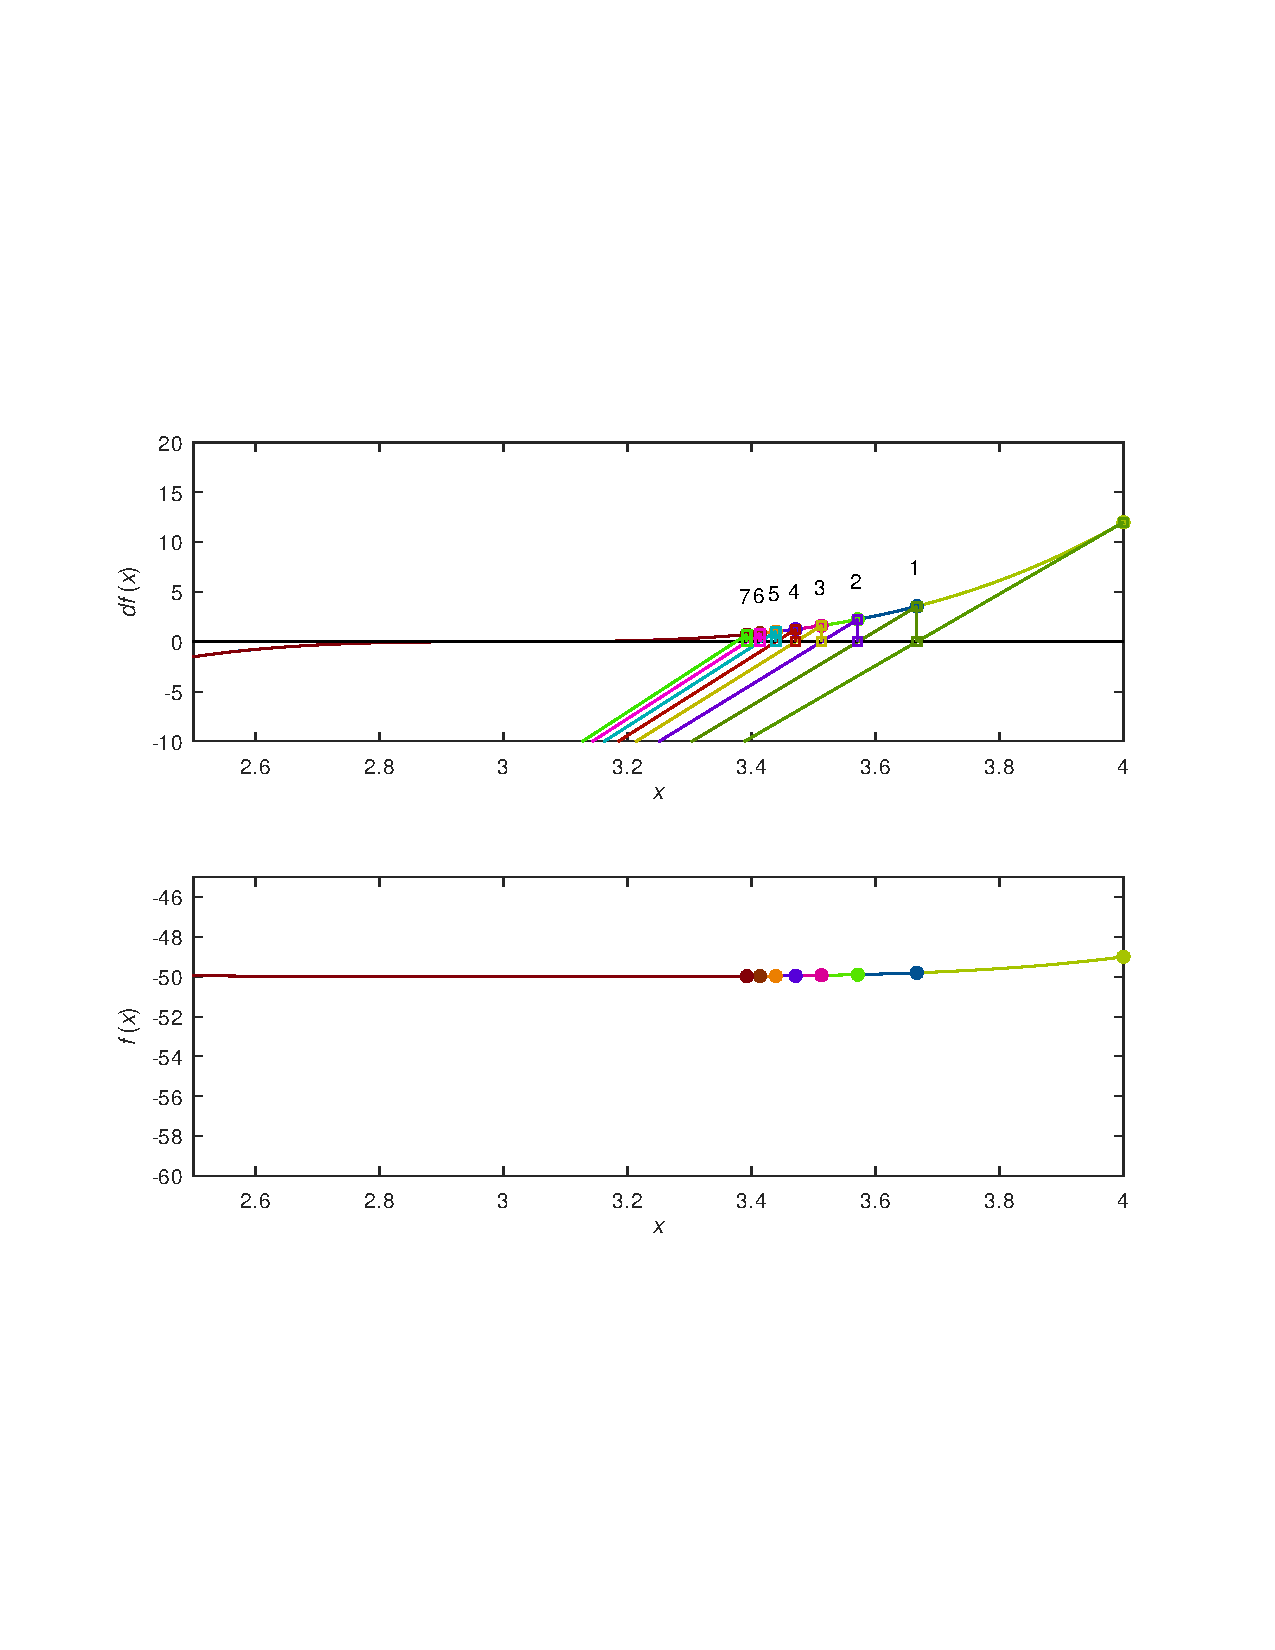
\includegraphics[scale=0.4]{7secantitter.pdf}
        \caption{Седьмая итерация}
    \end{figure}
\newpage
\subsection*{Вывод}
В результате выполнения лабораторной работы было выяснено, что 
метод Трёхточечного деления для нашей функции работает лучше, чем метод секущих.
\end{document}
